\graphicspath{{Img/ribbon/}}

\chapter{Ribbon manipulation}

    \section{Assignment}
        The manipulation with the rhythmic gymnastics ribbon was chosen to demonstrate the dynamic motion combined with the visual/tactile perception on the \CloPeMa\/ robotic testbed.

        A common task for a human rhythmic gymnast is to swing the metallic pole hanging on a ribbon with one hand and catch it with the other hand (see Figure~\ref{fig:HumanGymnast}, the left side). Another rhythmic gymnast task is fast back and forth movements causing the ribbon to form spirals and other shapes that are nice to watch (see Figure~\ref{fig:HumanGymnast}, the right side).

        \begin{figure}[h]
            \centering
            \begin{tabular}{ccc}
            \includegraphics[height=0.35\textwidth]{HumanGymnastPendulum.png}
            %
            & &
            %
            \includegraphics[height=0.35\textwidth]{HumanGymnastShapes.png}
            \end{tabular}
            \caption{Left: Rhythmic gymnast catches the pole. Right: Rhythmic gymnast swings the ribbon.}
            \label{fig:HumanGymnast}
        \end{figure}



       \CloPeMa\/ ``robot rhythmic gymnast'' should perform a similar scenario that is defined to be the following. It starts from the state, in which the robot holds the pole hanging on the ribbon in its left gripper.
%
       \begin{enumerate}\itemsep0pt
       \label{enu:InformalAssignment}
            \item Swing the left arm in a way that the pole and the ribbon start to swing as well.
            \item Grasp the pole with the right gripper using one of the sensors present in the gripper.
            \item Make sure the pole was grasped, is held properly and release the ribbon from the left gripper.
            \item Perform a few fast moves with the right arm so that the ribbon forms a certain shape nice to watch.
       \end{enumerate}


    \section{Analysis}
        In order to fulfill the proposed scenario given in Section~\ref{enu:InformalAssignment}, I had to check a few capabilities of the \CloPeMa\/ robot.

        \subsection{Available sensors in the gripper}
            The gripper contains tactile, light, magnetic and proximity sensor in its tip $T$ \cite{SalanskyGripper}.

            \begin{figure}[h]
            \includegraphics[width=0.3\textwidth]{GripperDesc.png}
            \centering
            \caption{Gripper description.}
            \label{fig:GripperDesc}
            \end{figure}

        \subsection{Verifying the ability to catch the swinging pole}

            I decided to use the light sensor to detect the swinging pole. The output of the light sensor, the relative intensity $h$, goes up as the pole approaches it. If the pole swings with the gripper positioned at the turning point of the swinging motion, two peaks appear at the output of the light sensor. The first one appears when the pole passes the tip $T$ of the gripper on its way inside and the second one on its way out (see Figure~\ref{fig:GripperDesc}). The threshold for detecting the pole was set to $h = 30$. The time between the two peaks was measured. Figure~\ref{fig:SwingMeasurement} shows the obtained results. The total time during which the pole was inside the gripper was estimated to be $t_p = \SI{520}{ms}$.


            \begin{figure}[h]
            \includegraphics[width=0.5\textwidth]{SwingMeasurement.png}
            \centering
            \caption{Swinging pole detection.}
            \label{fig:SwingMeasurement}
            \end{figure}

        \subsection{Gripper closing speed}
            In order to catch a swinging pole on a ribbon, the capabilities of the gripper have to be explored.

            To control how much the gripper opens, parameter $n$ is introduced. It controls the gripper on a percentage like basis: $n=100$ for a fully closed gripper and $n=0$ for a fully opened gripper.

            The gripper was set to maximum speed (gripper frequency was set to $f_g = 25,000$) and the times $t_c$ (worst-case) the gripper needs to open and close were measured. The results are shown in Table~\ref{table:GripperClosingSpeeds}.

            \begin{table}\centering
            \ra{1.3}
            \begin{tabular}{@{}ccc@{}}\toprule
            Gripper state & $n$ & $ t_{c}$ [ms] \\ \midrule
            full open & 0 & 600 \\
            full close & 100 & 850 \\
            half close & 50 & 420 \\
            \bottomrule
            \end{tabular}
            \caption{Gripper speed.}
            \label{table:GripperClosingSpeeds}
            \end{table}

            To be able to catch the pole, the gripper cannot be fully opened as it cannot close fast enough. The gripper has to be only half opened to be able to catch the pole.

        \subsection{Maximal speed of the \CloPeMa\/ robot}
            The experiments performed to determine the maximum speed of the robot are described in~\cite{WagnerMaxRobotSpeed}. The robot can move faster if the executed trajectory has a low control point density.

            The \CloPeMa\/ testbed robot moves the fastest when it is operated directly through its control system on a trajectories taught in by a teach pendant. If the robot is managed by a program through ROS, its speed is limited to 20\% of its maximum speed at the level of the robot control system. For this reason, the following experiments were performed directly on trajectories taught in by the \CloPeMa\/ researcher Libor Wagner. Firstly, the robot had to perform a back and forth motion along a straight line in a general direction in 3D space (i.e. involving the motion of many robot joints simultaneously) at its maximum speed while holding the pole and the ribbon. The result was that the whole robot started shaking considerably due to the huge changes in acceleration. For this reason, for performing fast motions I decided to move the robotic arm using only one (and preferably the last) joint to reduce the motion impact on the whole construction.

            The conclusion is that the needed fast motions (to swing the pole and to make fast motions with the ribbon) will be performed using one joint only. In addition, to perform back and forth motions only the start and end point of the trajectory will be used to reduce the point density. The resulting motions are thus arcs.

    \section{Robotic rhythmic gymnast}
        \subsection{Equipment}
            I had a \SI{6}{m} long gymnastic ribbon (see Figure~\ref{fig:GymnasticRibbon}) and two gymnastic poles  at my disposal. The blue pole is shown in Figure~\ref{fig:GymnasticPoles}, left side  and the white pole in Figure~\ref{fig:GymnasticPoles}, right side. The properties (length $d$, weight $m$ and diameter $\phi$) of the gymnastic poles are shown in Table~\ref{table:PoleProperties}. The diameter $\phi$ is measured at the point where the pole is grasped by the right gripper.

            \begin{figure}[h]
            \includegraphics[width=0.5\textwidth]{RibbonAdj.png}
            \centering
            \caption{Rhythmic gymnastics ribbon.}
            \label{fig:GymnasticRibbon}
            \end{figure}

            \begin{figure}
                \centering
                \begin{tabular}{cc}
                \includegraphics[width=0.39\textwidth]{BluePoleAdj.png}
                %
                &
                %
                \includegraphics[width=0.39\textwidth]{WhitePoleAdj.png}
                \end{tabular}
                \caption{Left: Blue rhythmic gymnastics pole. Right: White rhythmic gymnastics pole.}
                \label{fig:GymnasticPoles}
            \end{figure}


            \begin{table}[h]\centering
            \ra{1.3}
            \begin{tabular}{@{}cccc@{}}\toprule
            Pole & Length $d$ [cm] & Weight $m$ [g] & diameter $\phi$ [mm] \\ \midrule
            blue & 59 & 29 & 0.84\\
            white & 57 & 22 & 0.72\\

            \bottomrule
            \end{tabular}
            \caption{Properties of the rhythmic gymnastics poles.}
            \label{table:PoleProperties}
            \end{table}


        \subsection{Experimental setup}
            The system consists of the end of the robot arm (left one), the ribbon and the pole (see Figure~\ref{fig:PoleInit}).

            Based on the given assignment in Section~\ref{enu:InformalAssignment} I designed a flow chart (see Figure~\ref{fig:Workflow}). It is explained below. I estimated the swinging angles $\alpha$ and $\theta$, catching threshold $h_{catch}$ and recatching threshold $r_{recatch}$ experimentally.

            The swinging angle $\alpha$ and $\theta$ are defined according to Figure~\ref{fig:SwingingAngle}.

            \begin{figure}[h]
            \includegraphics[width=0.2\textwidth]{SwingingAngleDef.png}
            \centering
            \caption{Definition of the swinging angles $\alpha$ and $\theta$.}
            \label{fig:SwingingAngle}
            \end{figure}

            \begin{figure}
            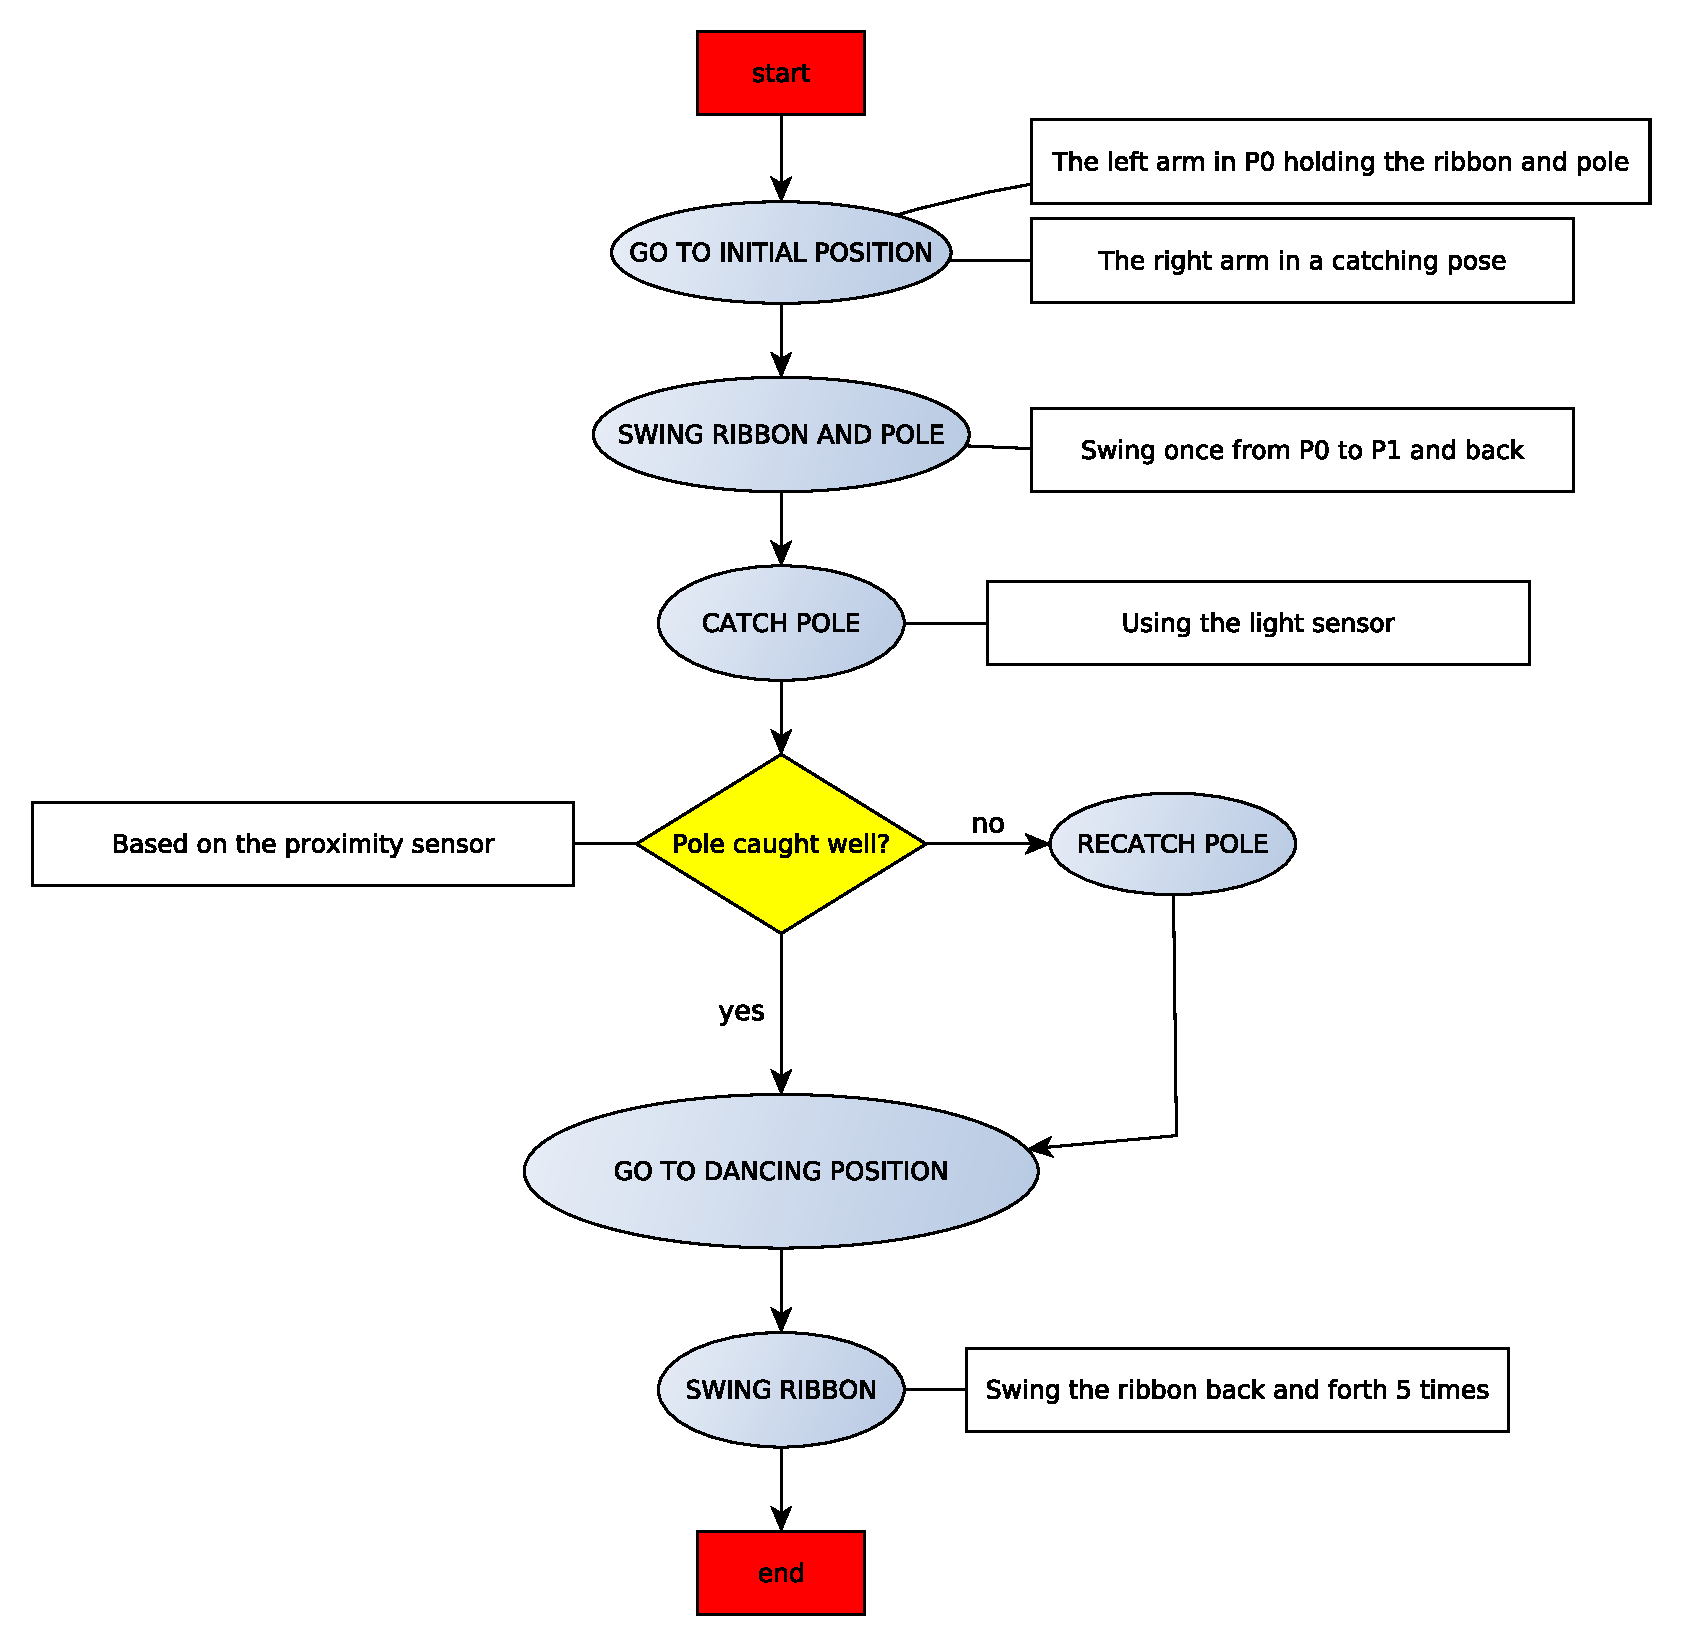
\includegraphics[width=0.9\textwidth]{PendulumWorkflow.pdf}
            \centering
            \caption{Robotic rhythmic gymnast workflow.}
            \label{fig:Workflow}
            \end{figure}

            \begin{figure}
                \centering
                \begin{tabular}{cc}
                \includegraphics[width=0.39\textwidth]{CaughtInsideAdj.png}
                %
                &
                %
                \includegraphics[width=0.39\textwidth]{CaughtWellAdj.png}
                \end{tabular}
                \caption{Left: The pole caught inside the gripper. Right: The pole caught well.}
                \label{fig:PoleCatching}
            \end{figure}

            \paragraph{INITIAL POSITION}~\\
                \noindent The right gripper holds the ribbon and the pole. The left arm is in the catching position. It means the right gripper should be positioned in the same plane in which the ribbon and pole swing. The turning point of the swinging motion should lie inside the gripper. It means that the pole should get inside the gripper at a certain point, but it should not hit the gripper.


            \paragraph{SWING THE RIBBON AND POLE}~\\
                \noindent The left robot arm swings back and forth between points $P_0$ and $P_1$ causing the pole and the ribbon to swing as well. The parameters $l = \SI{1}{m}$ and the swinging angle $\alpha = 22.5^o$ were used in experiments.

            \paragraph{CATCH THE POLE}~\\
                \noindent The right gripper starts closing from a half opened state as soon as the output of the light sensor exceed the closing threshold $h_{catch}=30$.

            \paragraph{Is the pole caught well?}~\\
                \noindent To determine whether the pole was caught inside the gripper (see Figure~\ref{fig:PoleCatching} Left) or caught well (see Figure~\ref{fig:PoleCatching} Right) the proximity sensor is used. If the recatching threshold exceeds $r_{recatch}= 5200$ an attempt to recatch the pole is made. It means that the gripper is opened for a short moment (to $n_{recatch}$) so that the pole moves towards its tip and closes back again ($n_{close}=100$) so that the pole stays inside the gripper.

            \paragraph{MOVE TO THE DANCING POSITION}~\\
                \noindent The left arm, which held the ribbon,  releases it and moves away. The right arm holding the pole moves up.

            \paragraph{SWING THE RIBBON}~\\
                \noindent The last joint of the right arm starts moving five times back and forth. The swinging angle is $\theta = 30.0^{o}$, so the total angle is two times bigger.


            \begin{figure}
            \includegraphics[height=0.4\textwidth]{PoleInit.png}
            \centering
            \caption{The hanging pole and the ribbon.}
            \label{fig:PoleInit}
            \end{figure}


        \subsection{Mathematical description of the swinging pole}

            My first idea was to describe the whole system mathematically as a double pendulum and then solve the appropriate differential equations. After that, I thought I would use the control theory to compute the motion of the left robot arm that will cause the maximum swinging amplitude of the pole hanging on the ribbon. However, after I finally came up with the system description using the Lagrange formalism, I realized that this approach is too complicated.

            For this reason, I tried to use the simplest description of a pendulum -- the mathematical pendulum (see Equation~\eqref{eq:MathematicalPendulum}).

            \begin{equation} \label{eq:MathematicalPendulum}
                \ddot{\varphi} = -\frac{g}{l}\sin(\varphi)
            \end{equation}

            The natural oscillations of a mathematical pendulum are described by Equation~\eqref{eq:T0}. In our case ($l = \SI{1}{m}$), $T_0 = \SI{2.01}{s}$.

            \begin{equation} \label{eq:T0}
                T_0 = 2 \pi \sqrt{\frac{l}{g}}
            \end{equation}

            I assumed that the swinging pole and ribbon resemble the mathematical pendulum (no damping, no air resistance, the whole mass concentrated only at the tip of the pendulum as a point mass, only small angle oscillations etc.). Thus, to achieve resonance and hence a maximal amplitude of the forced oscillations, the driving period of the robotic arm $T_r$ has to equal $T_0$.


        \subsection{Experiments}
            Based on the designed workflow (see Figure~\ref{fig:Workflow}), I made a video with two different gymnastic poles -- the white one and the blue one. It is called \textit{Gymnastics.mpg} and can be found on the attached CD. The end of the blue pole was wrapped in tape so that it is easier for a human to hold it and it was thicker than the end of the white pole.

            Although the swinging ribbon and the pole break almost all the assumptions connected with the mathematical pendulum, the experiments with the real swinging pole and ribbon show that the maximal amplitude increases as the period of the driving oscillations $T_r$ approaches $T_0$. Furthermore, the driving oscillations are applied in a way that the whole pendulum is swung by its end.

            Figure~\ref{fig:PoleCaught} shows the successful catching of the swinging white pole.

            \begin{figure}[h]
            \includegraphics[height=0.4\textwidth]{PoleCaught.png}
            \centering
            \caption{The white pole caught.}
            \label{fig:PoleCaught}
            \end{figure}



        \subsection{Discussion}
            The success rate of the pole catching depends on how the ribbon is held by the left arm. Since the gymnastic ribbon is \SI{6}{m} long it has to be folded so that the left gripper can hold it. However, the position of the plane in which the ribbon and pole will swing later greatly depends on how the gripper holds it. For this reason, the correct catching position of the right gripper has to be adjusted manually every time the ribbon is placed into the left gripper. However, once the catching position is properly adjusted, the success pole catching rate is > 90\%.

            In approximately 90\% of the cases the pole is caught inside the gripper and has to be recaught. In approximately 10\% of the cases the pole is caught well.

            The recatching parameter was determined experimentally. $n_{recatch\_white} = 80$ for the white pole and $n_{recatch\_blue} = 69$ for the blue pole (the thicker one). This parameter has to be set in advance by a human.

            The whole process runs fully automatically with the exception of setting $n_{recatch}$ and determining the correct catching position. The fact that I used two different poles of different thickness and weight shows the generality of the proposed solution.


\clearpage 